\begin{figure}[t]
\centering
    \begin{subfigure}[t]{0.45\textwidth}
    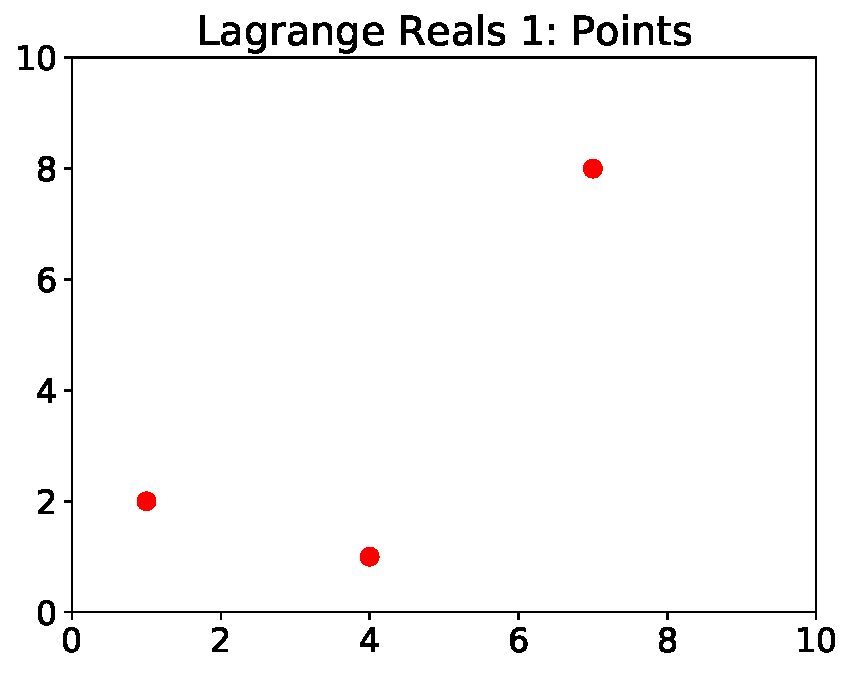
\includegraphics[width=\textwidth]{plots/lagrange/lagrange_reals_points_1.pdf}
    \caption{Lagrange interpolation data points}
    \label{fig:lagrange_points_1}
    \end{subfigure}
    \begin{subfigure}[t]{0.45\textwidth}
    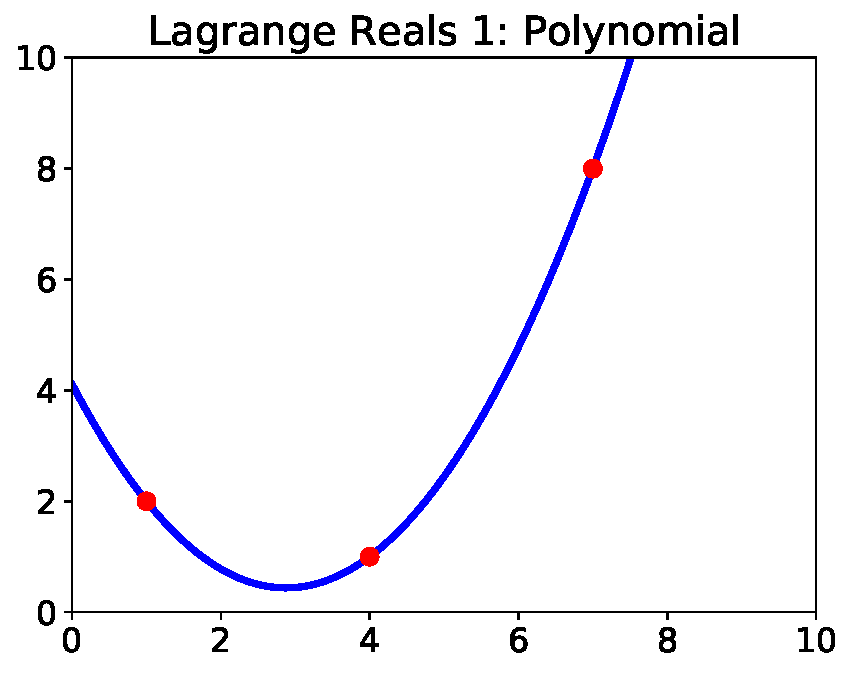
\includegraphics[width=\textwidth]{plots/lagrange/lagrange_reals_poly_1.pdf}
    \caption{Lagrange interpolation polynomial}
    \label{fig:lagrange_poly_1}
    \end{subfigure}
    \caption[Data points and Lagrange Interpolation over the reals 1]{Here
        are data points and Lagrange interpolating polynomial
        for Example~\ref{example:math_lagrange_reals_1}.}
\end{figure}

